\documentclass[a4paper,11pt]{ltjsarticle}
% 数式
\usepackage{amsmath,amsfonts}
\usepackage{bm}
% 画像
\usepackage{graphicx}
\usepackage{circuitikz}
\usepackage{amsmath,amssymb}
\usepackage{siunitx}
\usepackage{float}
\usepackage{tikz}
\usepackage{askmaps}
\usepackage{multirow}
\usepackage{bigstrut}
\usepackage{slashbox}
\usepackage{rotating}
\usepackage{listings}
% 数式
\usepackage{physics}
\usepackage{mathtools}
% 画像
\usepackage{subcaption}
% 表
\usepackage{makecell}
% その他
\usepackage{url}
\usepackage{ascmac}
\usepackage{cases}
\usepackage{here}
\usepackage{upgreek}
% 日本語対応
\usepackage{luatexja}
\usepackage{luatexja-fontspec}
\usepackage[top=1cm, bottom=2cm, left=2cm, right=2cm]{geometry}

\AtBeginDocument{\RenewCommandCopy\qty\SI}


\definecolor{commentgreen}{RGB}{0,200,0}
\definecolor{eminence}{RGB}{120,80,250}
\definecolor{weborange}{RGB}{255,165,0}
\definecolor{frenchplum}{RGB}{10,150,200}
\definecolor{commentgreen}{RGB}{0,200,0}
\definecolor{eminence}{RGB}{120,80,250}
\definecolor{weborange}{RGB}{255,165,0}
\definecolor{frenchplum}{RGB}{10,150,200}

\lstset{
        language = {C},
        basicstyle = \ttfamily\small,
        keywordstyle=\color{eminence}\ttfamily\bfseries,
        commentstyle=\color{commentgreen}\textit,
    identifierstyle=\color{black}\ttfamily,
        xleftmargin=.35in,
        frame=lines,
    showstringspaces=false,
        numbers=left,
        stepnumber = 1,
        breaklines=true,
        numberstyle = \ttfamily\normalsize,
    tabsize=4,  
        emph={int, int8_t, int16_t, int32_t, int64_t, uint8_t, uint16_t, uint32_t, uint64_t, char, double, float, unsigned, void, bool},
        emphstyle={\color{blue}}, 
        morekeywords={>, <, ., ;, +, -, *, /, !, =, ~},
        breakindent = 10pt, 
        framexleftmargin=10mm, 
        columns=fixed,
        basewidth=0.5em,
        }

% 特定のスタイル設定
\lstdefinestyle{customtxt}{
  basicstyle=\ttfamily\footnotesize,
  backgroundcolor=\color{lightgray},
  frame=single,
  breaklines=true,
  columns=fullflexible,
  showspaces=false,
  showstringspaces=false,
  showtabs=false,
  tabsize=4,
}

\newcommand{\fig}[4]{
    \begin{figure}[htbp]
      \centering
      \includegraphics{./image/#1}
      \caption{#2}
      \label{fig:#3}
    \end{figure}
  }
\begin{document}
\vspace*{-1cm}

\begin{center}
  {\Large \textbf{計算機アーキテクチャ \quad 中間演習課題}}
\end{center}

\vspace{0.2cm}
\begin{flushright}
  \underline{組番号\hspace{0.3cm}212\hspace{0.4cm}}\underline{氏名\hspace{0.7cm}古城隆人\hspace{0.8cm}}
\end{flushright}


\section{計算機で解ける問題と解けない問題のことを何というか答えなさい．}
計算可能性
\section{「クロード・シャノン」と「中嶋章」の 2 ⼈がほぼ同じ時代に考えだした理論を答えなさい．}
スイッチング理論
\section{計算機の第２世代の中⼼素⼦の名前と，開発した研究所の名前を答えなさい．}
トランジスタ，アメリカのベル研究所
\section{「AND /OR /NOT によるマルチプレクサ」の回路を⽰しなさい．}
図\ref{fig:multi}に示す．
\begin{figure}[H]
  \centering
  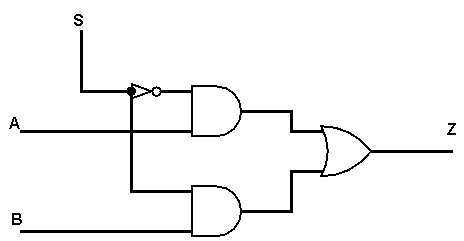
\includegraphics[width=10cm]{./image/multi.png}
  \caption{AND /OR /NOT によるマルチプレクサ}
  \label{fig:multi}
\end{figure}
\section{ 次の回路の論理式を答えなさい．}
\begin{math}
  \overline{(A+B) \cdot C + D \cdot E}
\end{math}
\section{ 以下の論理式の CMOS 回路を作成しなさい．}
図\ref{fig:cmos}に示す．
\begin{figure}[H]
  \centering
  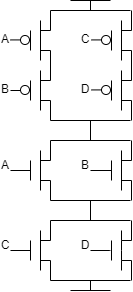
\includegraphics[width=3cm]{./image/CMOS_circuit.drawio.png}
  \caption{CMOS 回路}
  \label{fig:cmos}
\end{figure}
\section{下の図は何の回路を表すか答え名称を答えなさい．}
nMOSとpMOSを組み合わせた回路であり，制御入力が音の時に入力信号を出力信号として出力することが出来る回路である．
回路名は伝送ゲートである．
\section{10 進法で 8÷5=1 余り 3 を 2 進数の引き放し法で計算しなさい．}
以下のように計算を行い，余りが正のため，そのままで，商が 1，余りが $(3)_{10}$ となる．
\begin{table}[!ht]
  \centering
  \begin{tabular}{cccccccccccccc}
    ~ & ~ & ~ & ~ & ~ & 0 & 1 & 0 & 0 & 0 & ~ & ~ & ~ & ~ \\
    + & 1 & 1 & 0 & 1 & 1 & ~ & ~ & ~ & ~ & ~ & ~ & ~ & ~ \\ \hline
    ~ & 1 & 1 & 0 & 1 & 1 & 1 & 0 & 0 & 0 & ~ & ~ & ~ & 0 \\
    ~ & ~ & ~ & ~ & ~ & ~ & ~ & ~ & ~ & ~ & ~ & ~ & ~ & ~ \\
    ~ & 1 & 0 & 1 & 1 & 1 & 0 & 0 & 0 & ~ & ~ & ~ & ~ & ~ \\
    + & 0 & 0 & 1 & 0 & 1 & ~ & ~ & ~ & ~ & ~ & ~ & ~ & ~ \\ \hline
    ~ & 1 & 1 & 1 & 0 & 0 & 0 & 0 & 0 & ~ & ~ & ~ & ~ & 0 \\
    ~ & ~ & ~ & ~ & ~ & ~ & ~ & ~ & ~ & ~ & ~ & ~ & ~ & ~ \\
    ~ & 1 & 1 & 0 & 0 & 0 & 0 & 0 & ~ & ~ & ~ & ~ & ~ & ~ \\
    + & 0 & 0 & 1 & 0 & 1 & ~ & ~ & ~ & ~ & ~ & ~ & ~ & ~ \\ \hline
    ~ & 1 & 1 & 1 & 0 & 1 & 0 & 0 & ~ & ~ & ~ & ~ & ~ & 0 \\
    ~ & ~ & ~ & ~ & ~ & ~ & ~ & ~ & ~ & ~ & ~ & ~ & ~ & ~ \\
    ~ & 1 & 1 & 0 & 1 & 0 & 0 & ~ & ~ & ~ & ~ & ~ & ~ & ~ \\
    + & 0 & 0 & 1 & 0 & 1 & ~ & ~ & ~ & ~ & ~ & ~ & ~ & ~ \\ \hline
    ~ & 1 & 1 & 1 & 1 & 1 & 0 & ~ & ~ & ~ & ~ & ~ & ~ & 0 \\
    ~ & ~ & ~ & ~ & ~ & ~ & ~ & ~ & ~ & ~ & ~ & ~ & ~ & ~ \\
    ~ & 1 & 1 & 1 & 1 & 0 & ~ & ~ & ~ & ~ & ~ & ~ & ~ & ~ \\
    + & 0 & 0 & 1 & 0 & 1 & ~ & ~ & ~ & ~ & ~ & ~ & ~ & ~ \\ \hline
    1 & 0 & 0 & 0 & 1 & 1 & ~ & ~ & ~ & ~ & ~ & ~ & ~ & 1 \\
  \end{tabular}
\end{table}
\section{伝送ゲートは pMOS と nMOS を使っているが，なぜ pMOS だけではいけない理由を説明しなさい．}
nMOSトランジスタは，1の入力を，pMOSトランジスタは0の入力を出力側に通しにくい．そのため，
相補的にnMOSとpMOSを組み合わせることにより，両方の入力を正確に伝送できる．
\section{キャリールックアヘッド回路の利点と⽋点について説明しなさい．}
利点:加算器の速度を向上させることができる．
欠点:回路が複雑になり，設計と製造のコストが増加する．
\section{下の図は，何の回路を表しているか答え，A/L は何を⽰しているか答えなさい．}
8bitの右シフト回路であり，Aは算術シフト，Lは論理シフトの入力を示している．
\section{DRAM に対する SRAM の特徴を述べなさい．}
SRAMは高速であり，リフレッシュが不要であるが，DRAMに比べてメモリセルが大きいため，集積度が低い．
\section{ CAM について説明しなさい．}
CAM(Content Addressable Memory)は，回路上において検索したいデータをアドレスで返答するメモリの構造である．
メモリの出力と反転出力を用いて，検索データとメモリ内のデータを同時に比較し，
一致した場合に対応するアドレスを出力する．
一度にすべてのメモリを参照できるため，高速な検索が可能である．
\section{ハードウェアとソフトウェアのトレーオフとはどのような意味か説明しなさい．}
ハードウェアでは，柔軟性がないが高速であり，開発期間が延びる．
ソフトウェアでは，柔軟性があるが低速だが，開発期間が短縮される．
これらの長所と短所を考慮して，システム設計において最適なバランスを見つけることを指す．
\section{命令セットアーキテクチャの意味を説明しなさい．}
命令セットアーキテクチャ（ISA）は，マイクロプロセッサを動作させるための命令(オペコード)の集合と，
それらの命令がどのように動作するかを定義したものである．
\section{CPU は CISC 型と RISC 型に⼤別されるが，主にスマートフォン等に使⽤される CPU はどちらか．}
RISC 型
\section{アセンブリ⾔語レベルで，命令は⼤きく分けて 3 つに分かれるが，その 3 つを答えなさい．}
演算命令(算術演算、論理演算、シフト演算) ・ ロード/ストア命令(メモリ操作命令) ・ 分岐命令
\section{計算機の 1 つの命令を処理するステージとして，⼀般的な物を 5 つ挙げ，それぞれどんな処理をするかを答えなさい．}
フェッチ:命令をメモリから取得する．\\
デコード:取得した命令を解読し，必要な操作を特定する．\\
実行:命令に基づいて演算や操作を実行する．\\
メモリ:必要に応じてメモリからデータを読み取るか，書き込む．\\
ライト:演算結果をレジスタに書き込む．
\section{パイプラインとはどのような処理か，端的に説明しなさい．}
パイプラインは，命令を処理するときにstageごとに分解を行い，各ステージを並列に実行することで，
全体の処理速度を向上させる技術である．
\section{アムダールの法則とは何か端的に説明しなさい．}
アムダールの法則は，処理をいくら並列化しても，並列化できない部分の制約により，
全体の処理速度の向上には限界があることを示す法則である．
\section{バイパス機構とはどのような場合に役⽴つ機構か説明しなさい．}
バイパス機構は，$ ADD R_0 + R_1, R_2 $ 命令の直後に
$ ADD R_2 , R_3 , R_4 $ 命令が続く場合などに役立つ．
このような関係性をデータ依存性と呼び，バイパス機構では，
前の命令の結果をバッファを迂回して演算機へ直接渡すことで，
バイパスを実現している．
\section{浮動⼩数点形式において，正規化とはどのようなことか，例として単精度⽅式にて$(101.101)_2×2^2$ を正規化するとどう表されるかで説明しなさい．}
正規化とは，浮動小数点数の表現において，仮数部($F$)の値が1以上2未満になるように調整することを指す．
例を用いると，$(101.101)_2×2^2$が$(1.01101)_2×2^4$に正規化される．
\section{単精度⼩数点数の符号ビットを S，仮数ビットを F，指数ビットを E とすると，E=0 かつ F=0 の場合，どんな数として扱われるか答えなさい．}
ゼロとして扱われる．
\section{丸め処理に⽤いられるスティッキービットは何をするビットか説明しなさい．}
スティッキービットは，丸め処理において，切り捨てられたビットの中に1が存在するかどうかを示すビットであり，
丸めの決定に使用される．
\section{飽和演算とは何か説明しなさい．}
飽和演算は，演算結果が表現可能な範囲を超えた場合に，
最大値または最小値に固定する演算方法である．
\section{マルチメディア拡張機能とはどのような命令か端的に説明しなさい．}
画像や音声などの処理の際に，従来のALUのbit幅だとオーバースペックなため，
演算機内部に追加の回路を入れることにより32bitのめいれいはばのALUで8bitの演算を4個同時に並行で計算できるような
仕組みを持った命令である．
\section{プログラム内で変数を扱う場合，⼤域変数（グローバル変数）と局所変数（ローカル変数）があるが，迷った場合はどちらの変数を使⽤するべきか．また，その理由も説明しなさい．}
局所変数を使用するべきである．理由は，局所変数はサブルーチンが呼ばれない限りメモリを消費しないため，メモリの効率的な使用が可能となるためである．
\section{下の図は関数をどのように配置して処理するかを（a）〜（c）の 3 種類で⽰しているが，通常はどの⽅式で処理するか．また，その理由も説明しなさい．}
通常は(c)の方式で処理を行う．\\
理由として，(c)はメモリの効率的使用と実行速度の維持を両立させるためである．相対的なアドレスであるためポインタの計算が高速になるかつ，
関数の配置を呼び出したときにできるためメモリの使用効率もあげることができる．
\section{コールスタックとは何か端的に説明しなさい．}
サブルーチンを呼び出す際，引数や戻りアドレス，局所変数などの情報をレジスタに保存する場合，サブルーチンからサブルーチンを呼ぶ際など，レジスタの消費が速くなる．
そのため，これらのサブルーチンを呼ぶために必要な，復帰先命令アドレス/すたっくぽいんた/引き数/戻り値/極諸変数の各所場所を体系的に確保する構造である．
\section{バッファオーバーフロー攻撃を端的に説明しなさい．}
バッファオーバーフロー攻撃は，サブルーチンにおいて確保されているメモリサイズを超えるデータを書き込むことで，
隣接するメモリ領域を上書きし，悪意のあるコードを実行させる攻撃手法である．
\section{C ⾔語で gets が使われなくなった理由を説明しなさい．}
gets 関数は，入力されたデータの長さをチェックせずにメモリに書き込むため，
バッファオーバーフローの脆弱性を引き起こす可能性がある．
\section{Java 仮想マシンはコールスタックの仕組みの危険性を回避するため，どのような仕組みを⽤いているか答えなさい．}
Java 仮想マシンは，ヒープ領域とスタック領域にそれぞれ入出力可能なでーた構造と，極諸変数や戻り先アドレスを分離させることにより，
バッファオーバーフロー攻撃を回避している．
\section{メモリの内容をキャッシュに上げる場合の考え⽅を端的に説明しなさい．}
メモリの内容は，直近で使用する頻度が高いものをできるだけキャッシュに入れておきたいため，最近もっとも使われたキャッシュや，使用頻度などの観点からキャッシュにあげる
\section{キャッシュの 3 つのタイプの名称と，特徴を端的に答えなさい．}
1:ダイレクトマップ方式:メモリのブロックがキャッシュラインと一対一で紐づけられているタグ情報と比較され，検索を行う方式．\\
2:フルアソシアティブ方式:タグインデックスを用いず，キャッシュ内のすべてのラインとタグ情報を比較して検索を行う方式．\\
3:セットアソシアティブ方式:一つのタグインデックスに対して複数のタグ情報を持ち，その中で比較を行う方式．ダイレクトマップ方式では，一つのブロックにつき
一つのキャッシュラインしか対応できないが，セットアソシアティブ方式では，複数のキャッシュラインに対応できるため，キャッシュミスの発生率を低減できる．
\section{キャッシュミスを起こした場合の⼊れ替えアルゴリズムの種類を 4 つ答えなさい．}
ランダム，MRU，LRU，LFU
\section{キャッシュの内容と主記憶の内容の⼀貫性がなくなった時の対応⽅法に関して 2 つの⽅式を説明しなさい．}
ライトスルー方式: データがキャッシュに書き込まれると同時に主記憶にも書き込む方式．
ライトバック方式: データがキャッシュに書き込まれた後，
キャッシュから追い出されるときに主記憶に書き込む方式．
\section{分岐命令の分岐予測について，分岐命令ごとに分岐傾向を⽰す 2 ビットの表を何というか．}
PHT
\section{分岐命令の分岐予測について，⽤いられる GHR とはどのような動作をするか答えよ．}
直近に実行したN個の分岐命令の結果を格納したレジスタである．
\section{普通のキャッシュとトレースキャッシュの異なる点を端的に記述しなさい．}
トレースキャッシュは，アドレス順ではなく，命令の実行順にキャッシュに格納する方式である．
\section{データキャッシュにおいて，ノンブロッキングキャッシュについてどのようなものか説明しなさい．}
ノンブロッキングキャッシュは，キャッシュミスが発生しても，ブロックされずに
他の命令の実行を継続できるキャッシュ設計であり，
パイプラインの効率を向上させる．
\end{document}